\chapter{Segmentation}
Image segmentation is the process of dividing an image into meaningful non-overlapping regions or objects. The main goal is to divide an image into parts that have strong correalation with objects of the real world. Segmented regions are homogenous according to some property, such as pixel intensity or texture. Mathematically speaking, a complete segmentation of an image I is a finite set of regions \(I_1,...., I_S\) such that the condition (from \cite{drung00})
\begin{equation}
I = \bigcup_{i=1}^S I_{i} , \quad I_{i} \cap I_{j} = \emptyset , \quad i \neq j
\label{segCond}
\end{equation}
is satisfied. Image segmentation is one of the first steps leading to image analysis and interpretation. It is used in many different fields, such as machine vision, biometric measurements and medical imaging.

Automated image segmentation is a challenging problem for many different reasons. Noise, partial occluded regions, missing edges, lack of texture contrast between regions and background are some of the reasons. Noise is an artifact often found in images which makes the segmentation process harder. In the process of generating medical images noise is often introduced by the capturing devices. As a pre-processing step before segmentation the image can be smoothed to reduce noise. In the context of medical images segmentation usually means a delineation of anatomical structures. This is important for e.g. measurements of volume or shape. Low level segmentation methods are usually not good enough to segment medical images. Thus, higher level segmentation methods that are more complex and gives better results are used. Chapter 5-7 discusses some high level methods that can be used for segmentation, while this chapter will introduce a few simple segmentation methods. The biggest difference between low-level segmentation methods and higher level segmentation methods is the use of apriori information. Low-level methods usually have no information about the image to be segmented, while high-level segmentation methods can incorporate different types and amount of apriori information.

Traditional low-level image segmentation methods can roughly be divided according to the type of technique used:
\begin{itemize}
  \item Global/Histogram based methods
  \item Region based methods
  \item Edge based methods
\end{itemize}

\section{Histogram-based segmentation methods}
Global knowledge about an image is usually represented by the histogram of the intensity values in the image. Histogram-based segmentation methods uses this information to segment simple images. These segmentation methods are usually much faster than other methods, but restricted to images with simple features. 

\subsection{Thresholding}
The simplest segmentation approache is called thresholding. Thresholding is used to seperate one or more objects from the background and each other using one or more threshold values \(T\). A threshold value splits the image in two groups, where all pixels with intensity value higher than \(T\) represents one object, and the rest represents another object or the background. The threshold can be selected manually by either inspecting the image or the histogram of the image. A variety of methods for automatically selecting \(T\) exists. When little noise is present, the mean or median intensity values can be selected as the threshold. The simplest method to select a threshold, apart from doing it manually, is iterative thresholding and is computed as follows:
\begin{enumerate}
\item Choose an initial threshold \(T_{0}\) and segment the image.
\item The segmented image will consist of two groups, \(C_{1}\) and \(C_{2}\). Set the new threshold value \(T_{i}\) to be the sum of the mean intensity values from \(C_{1}\) and \(C_{2}\), divided by 2.
\item Segment the image using \(T_{i}\).
\item Repeat steps 2 and 3 until \(|T_{i} - T_{i-1}|\) is less than a predefined value.
\end{enumerate}
Images can be segmented into more than just two regions when thresholding by using more than one threshold value.
Segmentation by thresholding is only suitable for very simple images, where the objects in the image does not overlap and their intensity values are clearly distinct from the background intensity values.

\subsection{Otsu's thresholding method}
Otsu's thresholding method assumes that the image contains two regions with the values in each region creating a cluster. Otsu's method tries to make each cluster (or class) as tight as possible, thus minimizing their overlap. The goal then is to select the threshold that minimizes the combined spread. The threshold that maximizes the between-class variance \(\sigma_{b}^2(t) = \omega_{1}(t)\omega_{2}(t)\,[\mu_{1}(t)\mu_{2}(t)]^2\) is sought after. \(\omega_{1}(t)\) and \(\omega_{2}(t)\) are the weights (computed from the normalized histogram) of the two clusters, and \(\mu(t)\) is the mean intensity value of the clusters. Otsu's method starts by splitting the histogram into two clusters using an initial threshold. Then \(\sigma_{b}^2(t)\) is computed for that threshold value. The between-class variance \(\sigma_{b}^2(t)\) is then iteratively computed for every intensity value, and the threshold that maximizes the between-class variance \(\sigma_{b}^2(t)\) (or minimizes the within-class variance) is chosen as the final threshold value.

Figure \ref{thresholding} illustartes a gray-scale image and the segmentation results using both iterative global thresholding and Otsu's method. The threshold found using the iterative threshold method is 0.7332 where the range is from 0 (black) to 1 (white). The threshold found using Otsu's method is 0.7686. The image to be segmented is shown in figure \ref{thresholding}a, and its histogram in figure \ref{thresholding}b. As can be seen from the histogram, it is not possible to select a near perfect threshold by just looking at it. Figure \ref{thresholding}c illustrates the segmentation result from the iterative global thresholding method and figure \ref{thresholding}d is the segmentation result using Otsu's method. Even though the difference of the two threshold values is small, the segmentation results have a considerable difference, where Otsu's method gives a better result.

\begin{figure}[h!]
\centering
\begin{minipage}{.45\textwidth}
\begin{tabular}{c}
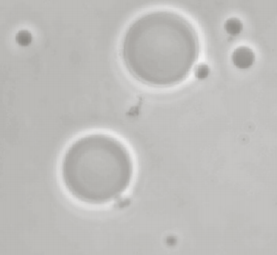
\includegraphics[width=.9\textwidth]{segmentation/NotSegmented} \\
(a)
\end{tabular}
\end{minipage}
\begin{minipage}{.45\textwidth}
\begin{tabular}{c}
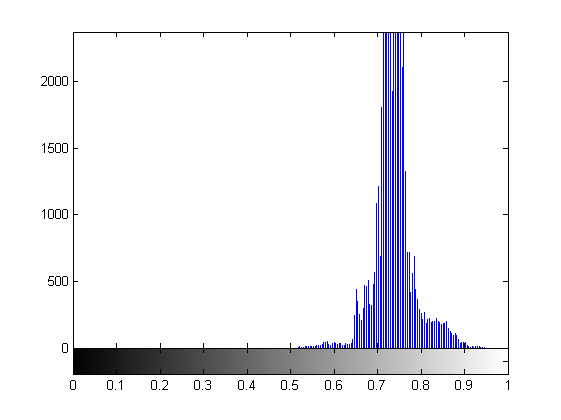
\includegraphics[width=.9\textwidth]{segmentation/NotSegmentedHist} \\
(b)
\end{tabular}
\end{minipage}
\\
\begin{minipage}{.45\textwidth}
\begin{tabular}{c}
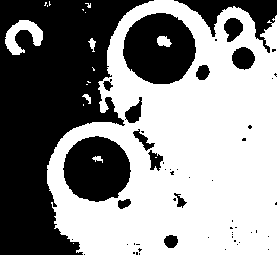
\includegraphics[width=.9\textwidth]{segmentation/globalThresholded} \\
(c)
\end{tabular}
\end{minipage}
\begin{minipage}{.45\textwidth}
\begin{tabular}{c}
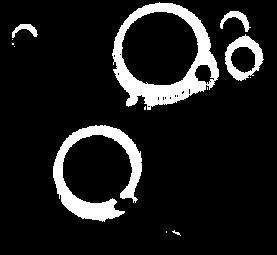
\includegraphics[width=.9\textwidth]{segmentation/otsuThresholded} \\
(d)
\end{tabular}
\end{minipage}
\caption{(a): Image to be segmented, (b): Histogram of image, (c): Segmented using iterative global thresholding, with $T = 0.7332$, (d): Segmented using Otus's method with $T = 0.7686$.}
\label{thresholding}
\end{figure}

\section{Region based segmentation}
Region based segmentation methods tries to find homogenous regions based on gray-scale, color, texture or any other pixel based measure in an image. Pixels with similar properties are grouped together in regions \(I_i\). The choice of homogenity criteria is an important factor that affects the end segmentation result. In addition to the condition in equation \ref{segCond}, images segmented by region based segmentation also satisfies the two following conditions:
\begin{itemize}
  \item All regions \(I_i\) should be homogenous according to some specified criteria: \(H(I_i) = true, \ i=1,2,...,S.\) \label{test}
  \item The region that results from merging two adjacent regions \(R_i\) and \(R_j\) is not homogenous: \(H(I_i \cup I_j) = false. \label{test2} \) 
\end{itemize}
An example of a homogenity criteria for a region could be all adjacent pixels with intensity value within a range \(\{x,y|x \pm y\}\). That is, if two adjacent pixels have intensity values in the range \(x \pm y\) they are in the same region. Region based segmentation methods are usually better than edge based segmentation methods in noisy images where the borders are difficult to detect. 

\subsection{Region growing}
The starting position of region growing (region merging) in the image is manually set at the beginning, and is called seed points. A seed point consiste of one or more pixels (voxels), and the region grow method starts by taking the image and seed points as input. A small region of 4x4 or 8x8 can for example be chosen as a seed region. The regions described by the seed points grows by merging with their neighbouring points (or regions) if the homogenity criteria is met. This merging is continued until merging any more would violate the homogenity criteria. When a region cannot be merged with any of its neighbours it is marked as final, and when all regions are marked as final the segmentation is completed. The result of region growing can depend on the order in which the regions are merged. Thus, the segmentation result may differ if the segmentation begins, for example, in the top right corner or the lower left corner. This is because the order of the merging can cause two similar adjacent regions \(R_1\) and \(R_2\) not to be merged if an earlier merge of \(R_1\) and \(R_3\) changed the characteristics of \(R_1\) such that it no longer is similar (enough) to \(R_2\). 

\subsection{Region splitting}
Region splitting is the opposite of region growing, and starts with a single region covering the whole image. This region is iteratively split into smaller regions until all regions are homogenous according to a homogenity criteria. One disadvantage of both region growing and region splitting is that they are sensitive to noise, resulting in regions that should be merged remaining unmerged, or merging regions that should not be merged.

\section{Edge based segmentation}
Edge based segmentation methods are used to find edges in the image by detecting intensity changes. The edge magnitude at a certain point is the same as the gradient magnitude, and the edge direction is perpendicular to the gradient. Thus, change in intensity at a point can be detected by using first and second order derivatives. There are various edge detection operators, and they all approximate a scalar edge value for each pixel in an image based on a collection of weights applied to the pixel and its neighbours. These operators are usually represented as rectangular masks or filters consisting of a set of weight values. These masks are applied to the image to be segmented using discrete convolution. 

\subsection{First and second order operators}
A simple second order edge detection operator is the Laplacian operator, based on the Laplacian equation:
\begin{equation}
\nabla^2f(x,y) = \frac{\partial^2 f}{\partial x^2} + \frac{\partial^2 f}{\partial y^2}
\end{equation}
This equation measures edge magnitude in all directions and is invariant to rotation of the image. Second order derivatives are commonly discretized by approximating it as \(\frac{\partial^2 f}{\partial x^2} = f(x+1,y) + f(x-1,y) - 2f(x,y)\) which is also how the Laplacian is discretized: 
\begin{equation}
\nabla^2f(x,y) = f(x+1,y) + f(x-1,y) + f(x,y+1) + f(x,y-1) - 4f(x,y)
\end{equation}
This Laplacian equation is represented by the mask in equation \ref{laplacianMask1}, and a variant of the equation that also takes into account diagonal elements is shown in \ref{laplacianMask2}.
\newline
\newline 
\begin{minipage}{.45\textwidth}
\begin{equation}
\begin{pmatrix}
0 & 1 & 0 \\
1 & -4 & 1 \\
0 & 1 & 0
\end{pmatrix}
\label{laplacianMask1}
\end{equation}
\end{minipage}
\begin{minipage}{.45\textwidth}
\begin{equation}
\begin{pmatrix}
1 & 1 & 1 \\
1 & -8 & 1 \\
1 & 1 & 1
\end{pmatrix}
\label{laplacianMask2}
\end{equation}
\end{minipage}
\newline
\newline

Since the Laplacian mask is based on second order derivatives it is very sensitive to noise. Moreover, it produces double edges and is not able to detect the edge direction. The center of the actual edge can be found by finding the zero-crossing between the double edges. Hence, the Laplacian is usually better then first order derivatives to find the center-line in thick edges. To overcome the sensitivity to noise problem, the image can be smoothed beforehand. This is the idea behind the Laplacian of Gaussian (LoG) operator. The LoG mask is a combination of a Gaussian operator (which is a smoothing mask) and a Laplacian mask. By convolving an image with a LoG mask it is smoothed at the same time as edges are detected. The smoothness is determined by the standard deviation of the Gaussian, which also determines the size of the LoG mask.

There are various masks based on first order derivatives, and two of them are the Prewitt and Sobel masks, represented in equation \ref{prew} and \ref{sobel} respectively. These two are not rotation invariant, but the masks can be rotated to emphasize edges of different directions. The masks as they are represented in equation \ref{prew} and \ref{sobel} highlights horizontal edges.
\newline
\newline
\begin{minipage}{.45\textwidth}
\begin{equation}
\begin{pmatrix}
1 & 1 & 1 \\
0 & 0 & 0 \\
-1 & -1 & -1
\end{pmatrix}
\label{prew}
\end{equation}
\end{minipage}
\begin{minipage}{.45\textwidth}
\begin{equation}
\begin{pmatrix}
1 & 2 & 1 \\
0 & 0 & 0 \\
-1 & -2 & -1
\end{pmatrix}
\label{sobel}
\end{equation}
\end{minipage}
\newline
\newline
As can be seen from the above masks, the only difference between the Sobel and Prewitt is that the middle column (or row in a rotated version) in the Sobel mask is weighted by 2 and -2. This results in smoothing since the middle pixel is given more importance, hence, the Sobel is less sensitive to noise than Prewitt. 

Figure \ref{edgeSeg}a illustrates a gray-scale image and \ref{edgeSeg}b is the edge segmented image based on LoG. \ref{edgeSeg}c is the edge image resulted from the Sobel mask in equation \ref{sobel}b and \ref{edgeSeg}d is the result from segmentation after rotating the mask \(90^\circ\). The segmentations resulted by using the Prewitt operator to segment the image in figure \ref{edgeSeg}a had no significant difference from the Sobel segmented images.

\begin{figure}[h!]
\centering
\begin{minipage}{.45\textwidth}
\begin{tabular}{c}
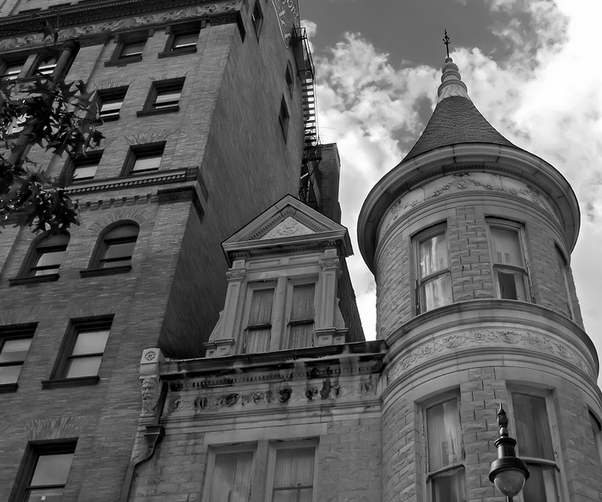
\includegraphics[width=.9\textwidth]{segmentation/Building} \\
(a)
\end{tabular}
\end{minipage}
\begin{minipage}{.45\textwidth}
\begin{tabular}{c}
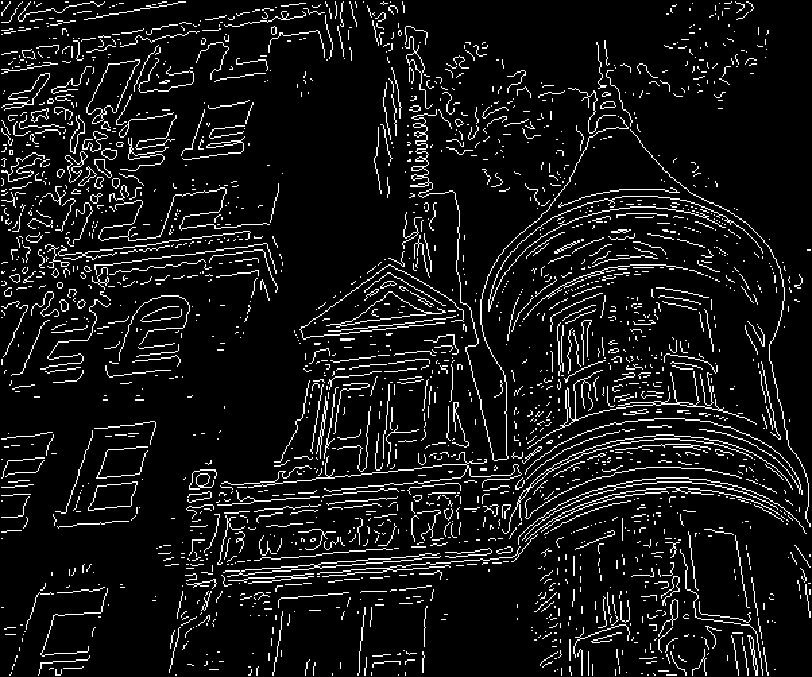
\includegraphics[width=.9\textwidth]{segmentation/LoG} \\
(b)
\end{tabular}
\end{minipage}
\\
\begin{minipage}{.45\textwidth}
\begin{tabular}{c}
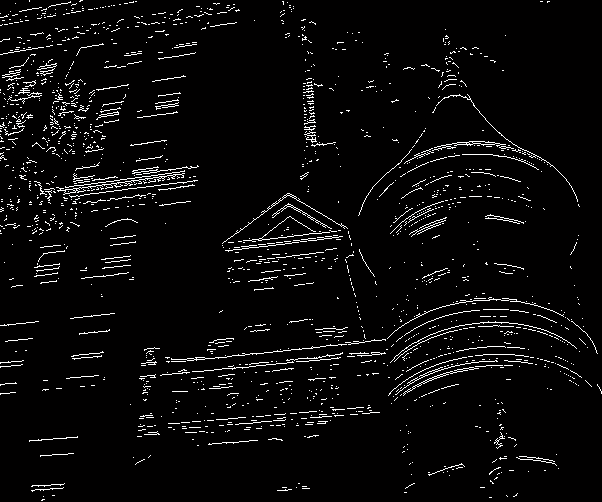
\includegraphics[width=.9\textwidth]{segmentation/sobelHorizontal} \\
(c)
\end{tabular}
\end{minipage}
\begin{minipage}{.45\textwidth}
\begin{tabular}{c}
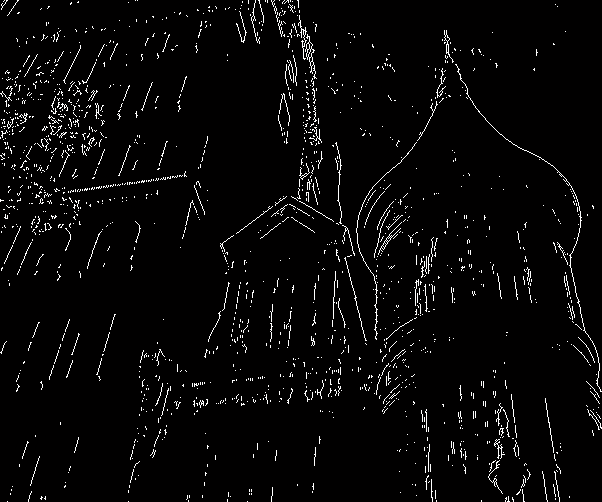
\includegraphics[width=.9\textwidth]{segmentation/sobelVertical} \\
(d)
\end{tabular}
\end{minipage}
\caption{(a): Image to be segmented, (b): LoG, (c): Sobel - highlighting horizontal edges, (d):Sobel - highlighting vertical edges}
\label{edgeSeg}
\end{figure}

\subsection{Canny edge detector}
A more powerful edge detection method is the Canny edge detector. This method consist of four steps. The first step is to smooth the image based on a Gaussian filter with a given standard deviation \(\sigma\). In the next step the derivatives in both directions are computed using any first order operator, and using these the gradient magnitude image and its direction are computed. The gradient magnitude image typically contains wide ridges around local maxima of the gradient. In order to get a single response to an edge, only local maxima should be marked as edges, and this process is called non-maxima suppression. A simple way for non-maxima suppression is to first quantize the edge directions according to 8-connectivity (or 4 connectivity). Then consider each pixel with magnitude \(> 0\) as candidate edge pixels. For every candidate edge pixel look at the two neighboring pixels in edge-direction and the opposite direction. If the magnitude of the candidate edge pixel is not larger than the magnitude of these neighboring pixels, mark the pixel for deletion. When all candidate edge pixels are inspected, remove all the candidates that are marked for deletion. Now all the edges will contain a single response, but there still are lines/pixels that are not part of any continues edge. To remove these, hysteresis thresholding is used. Hysteresis thresholding consist of segmenting the image with two threshold values. First, the non-maxima supressed images is thresolded with a high thresold value \(T_h\) that determines which of the remaining candidate edge pixels are immediately considered as edge pixels (strong edges). The high threshold value leads to an image with broken edge contours. Therefore a low thresold value \(T_l\) is used to threshold the non-maxima supressed image again. The pixels in this segmented image that are connected to a strong edge are added to the final edge image.

The Canny edge detector gives different results based on the values of \(\sigma\), \(T_h\) and \(T_l\), but the derivative operator used to find the magnitude and how the non-maxima suppression was implemented also affects the final edge segmented image.